\documentclass{article}
\usepackage[utf8]{inputenc}
\usepackage{enumitem}
\usepackage{geometry}
\usepackage{fancyhdr}
\usepackage{graphicx}
\usepackage{hyperref}

% document settings start
\newenvironment{problem}{\begin{enumerate}[label=\bfseries\alph*.]\large\bfseries}{\end{enumerate}}
\newenvironment{answered}{\par\normalfont}{}


\geometry{a4paper, margin=0.9in}
\graphicspath{{./outputs/}}

\pagestyle{fancy}
\lhead{Multimedia}
\rhead{Suman Mondal}
% \lfoot{\href{https://github.com/thatsuman/ccpcst-assignments.git}{View on Github}}
\rfoot{Page \thepage}

% \urlstyle{same}

% \newcommand{\problem}[2]{
  \subsection{#2}
    \underline{\emph{\Large Source Code :}}
    \inputminted[breaklines]{java}{#1.java}
    \bigbreak
    \noindent
    \underline{\emph{\Large Program Output :}}
    \bigbreak
    \noindent
    \includegraphics{#1}
\newpage
}

% document settings end

\begin{document}
\begin{titlepage}
  \begin{center}
    \vspace*{2cm}
    
\includegraphics[width=0.3\textwidth]{logo}\\
    \vspace{0.5cm}
    {\huge \textbf{CENTRAL CALCUTTA POLYTECHNIC}}\\
    \vspace{0.4cm}
    21, Convent Road, Philips, Sealdah, Kolkata, West Bengal 700014\\
    \vspace{0.8cm}
    {\Large \textsc{dept. : computer science and technology}}
  \end{center}
  \vspace{1.2cm}
  \textsc{
    \huge
    \begin{itemize}
      \item name : suman mondal
      \item roll : dccpcsts5
      \item number : 10005537
      \item reg number : d192005242
      \item subject : java programming
      \item session : 2021 - 2022
      \item email : suman.mondal@outlook.in
    \end{itemize}
  }

\end{titlepage}


% \newpage
% \tableofcontents
% \newpage

\section{Multimedia Assignment}

\noindent
    \begin{problem}
        \item Make Passport Size Photo and Discuss the Steps
            \begin{answered}
                \begin{itemize}
                    \item Import your image into Photoshop by going to File > Open 
                    
                    \item Now select your file from a flash drive or camera or in whichever storage device you have the image stored.
                    
                    \item Select the crop tool.With the crop tool selected, view the crop bar option at the top.Now in the drop-down options list that appears, select the 1x1 (Square) option.
                    
                    \item Drag the crop selector to include your shoulders and finish just above your hairline. To change the size of the cropped area, click and drag the corners, or click and drag anywhere within the cropped area to move it.
                    
                    \item The crop bar at the top will display the option to adjust the size after your 1x1 picture has been cropped. Once processed in Photoshop the image should adhere to the following standards by which the photo should be \textbf{3.5x4.5cm}.
                    
                    \item Select Image > Image size. The resolution should be 300.
                    Press CTRL+A to select all of the image and then hit CTRL+C to copy the image.
                    
                    \item Now navigate to Click Image and then to Canvas Size. Adjust the Canvas Size to 6in width by 4in height to print on 4x6 photo paper.
                    
                    \item Then click on the red block below to shift the first photo, click ok and CTRL+V to paste the copy of the photo. Finally, use the move tool to move the picture around in order to fit it.
                \end{itemize}
                \begin{center}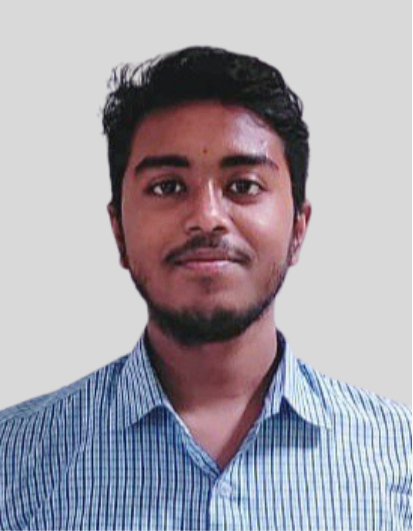
\includegraphics{./outputs/ps.png}\end{center}
            \end{answered}
        
        \item{Make Stamp Size Photo and Discuss the Steps} 
            \begin{answered}
                \indent
                    Same process as Passport Size photo only change the size to \textbf{2x3.25cm}
                    \begin{center}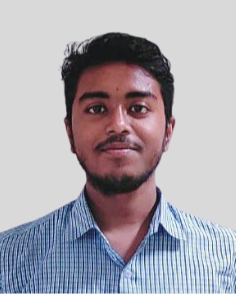
\includegraphics{./outputs/ss.png}\end{center}

            \end{answered}
        
        \item{Make a Collage and Discuss the Steps}
            \begin{answered}
                \begin{itemize}
                    \item Selected the Photos
                    \item Then I Opened the ‘New Document’ panel in Photoshop and chose a horizontal A4 size at 72 PPI.
                    \item Created the first vertical guide. Chose View > New Guide. In the dialog box, I selected Vertical orientation, entered 450 px position and click OK.  Repeat this step for position 900 px. croped the grids as per needs.
                    Now create a horizontal guide. Choose View >New Guide. In the dialog box, select Horizontal orientation, enter 450 px position and click OK. Repeat this step for position 900 px. To see the guidelines, then choose View > Show > Guides. 
                    for lock all guides, choose View >Lock Guides.
                    \item Added the Images using drag and drop.
                    \item Crop and resized them as per grids
                    \item Added the Text by using Text Box
                \end{itemize}
                \begin{center}\includegraphics[height=3.2in,width=4.3in]{./outputs/clg2.png}\end{center}
            \end{answered}


    \end{problem}

\end{document}

